\documentclass{beamer}
\usepackage[utf8]{inputenc}
\usepackage[frenchb]{babel}
\usepackage{tikz}
\usepackage{subfigure}
\usepackage[scriptsize]{caption}
\usepackage{multicol}
\renewcommand*{\figurename}{}
\usetikzlibrary{shapes,positioning,snakes,calc}
\usetheme{Darmstadt}
\usepackage{graphicx}

% \setbeamercolor{alerted text}{fg=blue}

\title{FMIN327 Cognition individuelle et collective\\ Protocoles artificiels entre agents naturels}
\author{DUPÉRON Georges \and\\ BONAVERO Yoann}
\institute{Université Montpellier II, Département informatique  \\ Master 2 IFPRU \\ Sous la direction de Monsieur Jacques Ferber}
\date{Jeudi, 3 novembre 2011}

\defbeamertemplate*{footline}{shadow theme}
{%
  \leavevmode%
  \hbox{\begin{beamercolorbox}[wd=.5\paperwidth,ht=2.5ex,dp=1.125ex,leftskip=.3cm plus1fil,rightskip=.3cm]{author in head/foot}%
    \usebeamerfont{author in head/foot}\insertframenumber\,/\,\inserttotalframenumber%\hfill\url{http://www.pticlic.fr/}
  \end{beamercolorbox}%
  \begin{beamercolorbox}[wd=.5\paperwidth,ht=2.5ex,dp=1.125ex,leftskip=.3cm,rightskip=.3cm plus1fil]{title in head/foot}%
    \usebeamerfont{title in head/foot}\insertshorttitle%
  \end{beamercolorbox}}%
  \vskip0pt%
}

\begin{document}
\renewcommand*{\figurename}{}

\begin{frame}
  \titlepage
\end{frame}

\section{Introduction}

\begin{frame}
Approche globale :
\\ Tout individu quel qu'il soit, privé de toutes formes de communication, d'émotions et de sensations, ne peuvent
en aucune manière évoluer et former de groupes cohérents. La cohérence et l'intégrité d'un groupe passe majoritairement
par un échange d'informations entre les individus. Celles-ci ne peuvent pas être transmises n'importe
comment, les individus constituant le groupe doivent être en mesure de les comprendre.
\\ Le formatage de l'information devient essentiel tout comme le support qui va être utilisé.
\newline 
\end{frame}

\begin{frame}
Définitions :
\begin{itemize}
	\item Protocoles artificiels
	Définition de manière tout à fait artificielle d'un ensemble de règles.
	\item Agents naturels
	Tous types d'individus "naturels", individus non engendrés par une action humaine (A revoir).
\end{itemize}
\end{frame}

\begin{frame}
Les limites :
\begin{itemize}
	\item Les protocoles artificiels formels
	\item Autres limites
\end{itemize}
\end{frame}

\section{Espéranto}

\begin{frame}
\begin{center}
\huge Espéranto
\end{center}
\begin{itemize}
\item Origine et but.
\item Une langue dite "construite"
\end{itemize}
\end{frame}

\begin{frame}
\begin{center}
\huge Espéranto
\end{center}
\begin{itemize}
\item Une grammaire régulière.
\\ Exemple
\item Une langue "agglutinante".
\\ Exemple.
\end{itemize}
\end{frame}

\begin{frame}
\begin{center}
\huge Espéranto
\end{center}
Une langue vivante.
\\ Petit paragraphe en espéranto.
\end{frame}

\section[Contrats]{Législation et contrats formels}

\begin{frame}  
  \begin{itemize}
  \item Brouillon de spec
  \item Pas d'implémentation
  \end{itemize}
\end{frame}

\section{Supports}

\begin{frame}  
  \begin{itemize}
  \item Alphabet % + origine de l'alphabet
  \item Morse
  \item Braille
  \item Langage des signes
  \end{itemize}
\end{frame}

\begin{frame}  
  \Huge Alphabet
\end{frame}


\begin{frame}
  \Huge Le morse :
  \normalsize \begin{itemize}
  \item Invention attribué à Samuel Morse (1791 - 1872)
  \item Créé en 1835
  \item Seulement deux types d'impulsion sont nécessaires.
  \end{itemize}
  % Ajouter la photo de Samuel Morse.
\end{frame}

\begin{frame}  
  \Huge Le morse.
  \\ \normalsize Un exemple Alphabet écrit en morse.
\end{frame}


\begin{frame}  
  \Huge{Le braille}
  \begin{center}
  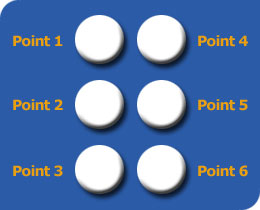
\includegraphics[width=4cm]{./include/cellule_braille.jpg}
  \end{center}
  \normalsize \begin{itemize}
  \item Louis Braille (1809 - 1852)
  \item Inventé en 1824
  \item Alphabet en relief
  \item 64 combinaisons pour tout faire
  \end{itemize}
\end{frame}

\begin{frame}  
  \Huge Le braille
  \\ des exemples.
\end{frame}


\begin{frame}  
  \Huge La langue des signes.
\end{frame}

\begin{frame}  
  \Huge La langue des signes.
\end{frame}

\section{Procédures administratives}

\begin{frame}
\end{frame}

\section{Conclusion}

\begin{frame}
  \begin{itemize}
  \item Sujet ouvert% 0 résultats sur google pour "protocoles artificiels" "agents naturels".
  \end{itemize}
\end{frame}

\end{document}
